% A simple Pentagon with TiKZ
% Author: Christoph Gerum <gerum@informatik.uni-tuebingen.de>

\documentclass{article}

\usepackage{tikz}


\begin{document}

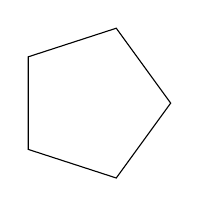
\begin{tikzpicture}
%  \draw [step=0.25cm,color=gray] (-1, -1) grid (1, 1);
  
  \path (0,0) coordinate (P0);
  \path (0*72:1cm) coordinate (P1);
  \path (1*72:1cm) coordinate (P2);
  \path (2*72:1cm) coordinate (P3);
  \path (3*72:1cm) coordinate (P4);
  \path (4*72:1cm) coordinate (P5);

  \draw (P1) -- (P2) -- (P3) -- (P4) -- (P5) -- cycle;

\end{tikzpicture}


\end{document}
